\subsection{Route-Specific Lifecycles and Evidence}
\label{sec:routes}
\label{sec:mech}
\label{sec:objective}
\label{sec:nodeexec}
\label{sec:ack}

\paragraph{Timing and approval}
Timing guards are route-specific. Online node writes enforce an effective
minimum spacing of 60\,s. Recipe dispatch uses a per-recipe interval anchored
to approval, while trials also use a configurable per-line cadence (default
300\,s). The recipe interval can refuse a proposal before an approval request
is created. Checks occur at proposal or execution according to the operation,
and experiment-specific pacing overrides are reported with the corresponding
results.

Manual bindings create an approval request containing the actor, operation,
candidate values, applicable limits, expiry, parameter bases, and the active
line--product--recipe--run context. The default wait expires after 180\,s and
refuses execution. After approval, the executor rechecks authorization and
compares the current context tuple with the approved tuple. For approved
recipe writes and dispatched rollback, a final synchronous comparison follows
the asynchronous grant check immediately before entering the DCW dispatch
path. Changes visible at this software boundary are refused before a driver
write. This check is not an atomic lock across network or device I/O and
cannot cancel a driver call after it begins. A focused mock-state suite
changes line, product, recipe, or run during approval for recipe apply, trial,
and dispatching rollback; each mutation is refused before a driver write or
new execution record. For
\texttt{recipe\_apply}, a changed recipe definition also requires a new
proposal; an unchanged approval dispatches a copy of the approved parameter
snapshot. A line-level recipe mode defaults to manual; changing it to
automatic requires administrator confirmation. The approval record
authorizes a workflow action and does not replace process protection.

Fig.~\ref{fig:hitl}(a) illustrates the four-layer interval in
Eq.~(\ref{eq:admission}) with an archived RPM configuration; panel (b) shows a
symbolic approval followed by context and authority rechecks. The plotted
values are illustrative and are not R20 measurements.

\begin{figure*}[!t]
\centering
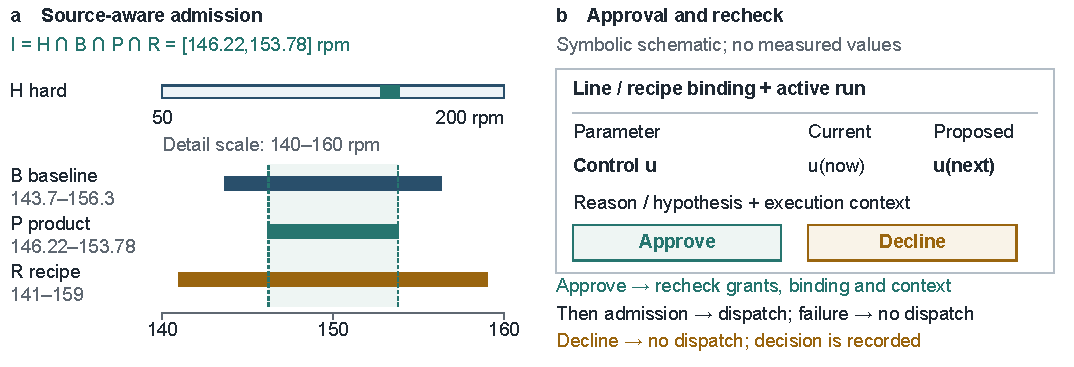
\includegraphics[width=\textwidth]{resources/fig-admission-hitl-2026.pdf}
\caption{Admission and approval boundaries. (a) Illustrative archived RPM
configuration (not part of R20):
online node interventions use the four-layer value interval of
Eq.~(\ref{eq:admission}),
whereas recipe dispatch omits the prior recipe window. (b) Symbolic human
approval binds a proposed action and its context tuple; execution rechecks the
active line--product--recipe--run context, authority, and applicable limits
after approval. Approval does not reserve equipment state.}
\label{fig:hitl}
\end{figure*}

\paragraph{Node probe}
The bounded \texttt{optimization\_explore} route is exposed to the AML
optimization profile. It validates a bound control and DAQ scope, captures a
baseline, routes a bounded write through DCW, and stores a later target window
as a separate exploration summary. Its timing and approval behavior is
route-specific; R20 does not exercise this route.

\paragraph{Recipe operations}
\texttt{recipe\_trial} checks the bound recipe and active run, then dispatches
candidate overrides as a batch with per-parameter verification. The caller
subsequently queries DAQ and may save a definition with
\texttt{recipe\_update}, restore one with \texttt{recipe\_rollback}, or apply
a version with \texttt{recipe\_apply}. A trial does not save or apply a
version, and endpoint verification is not a process-response measurement.
Public direct-node control is closed; bounded probes and recipe operations are
the configured write surfaces.

\paragraph{Command verification}
Command confirmation and process response answer different questions. A
driver ACK is graded as \texttt{readback-verified}, \texttt{transport-ack},
or \texttt{unverified}; a matching endpoint read supports the first grade,
whereas transport or MES application confirmation supports the second.
Recipe-batch verification is \texttt{verified}, \texttt{unverified}, or
\texttt{failed}. If readback is absent or mismatched, up to three reads are
attempted 2\,s apart. Initial ACKs, final ACKs, and per-parameter verdicts are
retained separately. A readback-verified setpoint does not establish target
attainment.

\paragraph{Observation, verdict, and compensation}
Recipe-path observation follows batch dispatch, and saving a definition,
applying it, and observing process response remain separate operations. An
open node record can request rollback after repeated breaches; missing samples
do not count as breaches. Caller verdicts and compensation remain separate
from the observation and subject to admission checks.
\label{sec:agentloop}
